\section{Division into objects}

To assure real modularity of our template, more divisions were proposed than only the one mentioned at the beginning of this chapter; their structure being represented in Figure \ref{objectStructure}.

We already mentioned the separation of the Algorithm from the State Space. It is useful to think of the Algorithm as of a decision-maker. Its role is restricted to making decisions on acceptance or rejections of the proposals generated by the State Space. However, the information on which it bases its decision depends on the points from the State Space indirectly, via the evaluations of densities ( or, in the discrete case, probability functions ) at these points. So we can see appear a third candidate for an entity - namely an object whose methods would serve to measure some characteristic of the State Space sample points. We call this entity the Target Measure. 

The idea behind the Target Measure entity is that of containing user-defined probability function or a density together with every additional data-structure required for its calculation. If the user were interested in simply evaluating the \PT's potential on some toy-example that was analytically tractable or could be simulated using any other simpler and more efficient technique, the Target Measure entity would be the place to store any additional methods tied with the particular distribution. For example, in the present research (confront Chapter \ref{simulationsAndResults}) we could  additionally provide an efficient method for quantile simulations and evaluate the real distribuant. 

\begin{figure}
	\centering 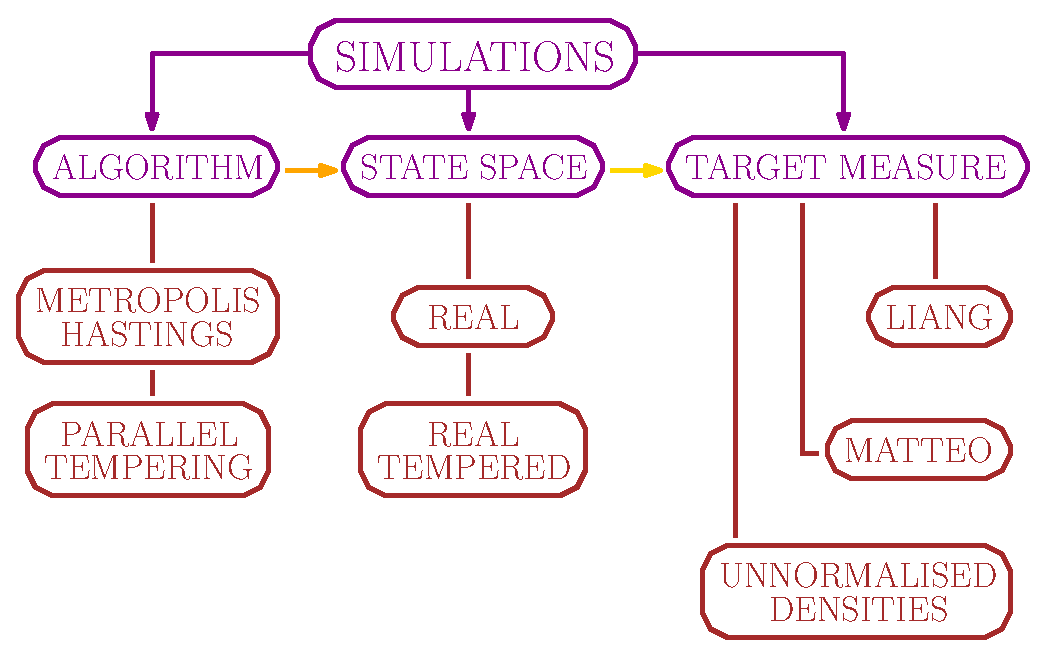
\includegraphics[keepaspectratio=true, width =\linewidth]{./img/objectStructure.eps}
	\caption{Division of our programme into operational objects.}\label{objectStructure}
\end{figure}

The question remains, are there any significant differences between the State Space and Target Measure.